% Versión inicial de la investigación sobre los componentes software.

\section{Arquitecturas de \emph{software}}

Según \cite{taylorSoftwareArchitectureFoundations2009}, la \textbf{arquitectura de un sistema \emph{software}} es el conjunto de todas las \textbf{decisiones principales de diseño} que se toman durante su ciclo de vida; aquellas que sientan las bases del sistema. Estas afectan a todos sus apartados: la funcionalidad que debe ofrecer, la tecnología para su implementación, cómo se desplegará, etc. En conjunto, definen una pauta que guía (y a la vez refleja) el diseño, la implementación, la operación y la evolución del sistema.

Estudiar la arquitectura de un sistema nos permite conocerlo en profundidad. Nos permite descubrir qué \textbf{componentes} la conforman, cómo están \textbf{relacionados} y el por qué de esta composición. \cite{perryFoundationsStudySoftware1992} \textcolor{red}{Además, nos provee de un vocabulario común para que los \emph{stakeholders} o interesados puedan comunicarse: ayuda a los clientes a articular sus necesidades; a los diseñadores a capturar los requisitos y definir el sistema; a los desarrolladores a comprender mejor cómo implementarlo\dots}

Todos los sistemas \emph{software} cuentan con una arquitectura. La diferencia radica en si esta ha sido diseñada y descrita explícitamente o ha quedado implícita en su implementación. \cite{taylorSoftwareArchitectureFoundations2009} En el segundo caso es probable que, con el paso del tiempo, se ``erosione`` su arquitectura: se implementan funcionalidades sin respetar la estructura. También se olvida el por qué de ciertas decisiones. En general, se vuelve más difícil de mantener. Se convierte en una ''gran bola de barro''. \cite{footeBigBallMud1997}

Por tanto, es vital dedicar tiempo para definirla atendiendo a las necesidades de nuestro sistema. Una buena arquitectura es capaz dotar de estructura a nuestro sistema. \cite{martinCleanArchitectureCraftsman2018} Mientras se respete la arquitectura, y se mantenga actualizada, esta estructura Una buena arquitectura nos ofrece una serie de ventajas, como facilitar su desarrollo, mayor extensibilidad.

\subsection{Decisiones principales de diseño}

Las \textbf{decisiones principales de diseño} son todas aquellas decisiones importantes que afectan a los fundamentos de nuestro sistema. Son principales o importantes porque comienzan a ``asentarse`` cuando avanza el desarrollo. Se vuelven más difíciles de cambiar o rectificar. \cite{taylorSoftwareArchitectureFoundations2009} Estas decisiones no solo se toman durante la concepción del sistema, si no que también pueden surgir durante el desarrollo y posterior evolución.

Normalmente se resumen en comparativas entre distintas alternativas, cada una de ellas con sus ventajas e inconvenientes. Por ejemplo, una decisión de diseño principal que se suele tomar en las fases tempranas del desarrollo es la elección de la topología para la solución. Optar entre desarrollar un servicio monolítico, o un sistema formado por microservicios, va a condicionar prácticamente todo el desarrollo.

Aun así, no todas las decisiones de diseño tienen por qué ser consideradas como principales. Hay detalles de implementación que pueden dejarse ambiguos a nivel de la arquitectura. Se concretarán durante en el momento en que se implementen.

 Pueden tomarse en base a distintos criterios. Entre ellos podemos destacar: \textcolor{red}{[Citation needed]}

    \begin{itemize}
        \item \textbf{Requisitos del sistema:} a partir del dominio y las necesidades de nuestros usuarios, podemos deducir: la funcionalidad a implementar, las restricciones que debemos respetar y otras propiedades que debe poseer el sistema.

        \item \textbf{Arquitectura actual:} las decisiones tomadas previamente también condicionan las elecciones que se tomen más adelante. Cuanto más avanza el desarrollo, más se asientan las decisiones previas, y más dificil es rectificarlas.

        \item \textbf{Experiencia previa:} del desarrollo de este u otros sistemas. Podemos obtener métricas del funcionamiento y uso de nuestro sistema para informar decisiones futuras. \textcolor{red}{[Cita devops]}
    \end{itemize}

\subsection{Componentes de una arquitectura}

Otra posible definición de arquitectura la encontramos en el estándar IEEE 42010-2011 \cite{ieeeStandard420102011Systems2011}: es "\emph{un conjunto de conceptos o propiedades fundamentales, personificados por sus elementos, sus relaciones, y los principios que guían su diseño y evolución}".

Podemos describirlas usando tres conceptos: \cite{perryFoundationsStudySoftware1992}

    \begin{itemize}
        \item \textbf{Elementos}: Son las piezas fundamentales que conforman el sistema. Implementan la funcionalidad de la aplicación. Se utilizan para describir \emph{qué} partes componen el sistema. Por ejemplo: un módulo, un servicio web...

        \item \textbf{Forma}: El conjunto de propiedades y relaciones entre los elementos o el entorno de operación. Describe \emph{cómo} está organizado el sistema. Por ejemplo: un servicio contacta con otro a través de una API.

        \item \textbf{Justificación}: Razonamiento o motivación de las decisiones que se han tomado. Responden al \emph{por qué} algo se hace de determinada forma. Normalmente no pueden deducirse a partir de los elementos y la forma, por lo que es necesario describirlos.

    \end{itemize}

\pagebreak

\subsubsection{Elementos}

Durante el diseño del sistema, para lidiar con la complejidad que pudiera alcanzar, recurrimos a dos herramientas: la abstracción y la separación de responsabilidades. \cite{martinCleanArchitectureCraftsman2018} Aplicándolas repetidamente mientras estudiamos el espacio del problema pueden sernos de gran ayuda para identificar distintas unidades de funcionalidad. Se trata de los componentes.

Según \cite{taylorSoftwareArchitectureFoundations2009}, los \textbf{componentes} son ``elementos arquitectónicos que encapsulan un subconjunto de la funcionalidad y/o de los datos del sistema``.
Dependiendo de las características de nuestro sistema (y del nivel de abstracción que usemos) pueden tomar distintas formas: módulos dentro un mismo proceso, servicios distribuidos, etc.

\begin{wrapfigure}{r}{0.40\linewidth}
  \centering
  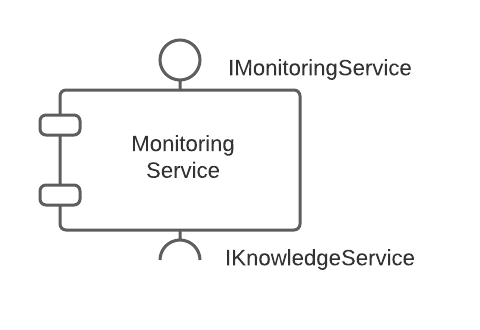
\includegraphics[scale=0.8]{03_arquitectura/images/componente-ejemplo}
  \caption{El servicio de monitorización representado como un componente. Ofrece una interfaz (\emph{IMonitoringService}) y depende de otra para funcionar (\emph{IKnowledgeService}).}
  \label{fig:componenteEjemplo}
\end{wrapfigure}

Los componentes exponen una \textbf{interfaz} que permite acceso a esa funcionalidad o datos que encapsulan. A su vez, también declaran una serie de \textbf{dependencias} con interfaces de otros componentes que requieren para operar. En la figura \ref{fig:componenteEjemplo} tenemos un ejemplo.

Por si solos, estos componentes independientes no aportan mucho valor. En lugar de eso, son la unidad básica de composición. Podemos conectar distintos componentes para que trabajen conjuntamente y realicen tareas más complejas. De esta forma podemos \textbf{componer sistemas}. Un aspecto clave es la integración y la interacción entre componentes. \cite{mehtaTaxonomySoftwareConnectors2000}

Para que dos o más componentes puedan interactuar, necesitamos definir un mecanismo de comunicación. Recurrimos entonces a los \textbf{conectores}: se trata de elementos arquitectónicos que nos ayudan a definir y razonar sobre la comunicación entre componentes. Representan la transferencia de datos y de control entre ellos. En la figura \ref{fig:componentesYConectorEjemplo} mostramos una representación de la necesidad de comunicación entre dos componentes a través de un conector. No se ha especificado todavía ningún detalle sobre cómo se implementará. Así, podemos estudiar la arquitectura y elegir los mecanismos adecuados para cada interacción del sistema. \cite{taylorSoftwareArchitectureFoundations2009}.

%% TODO: Los conectores son application-independent. No dependen de la funcionalidad de la aplicación.
%% TODO: Hablar de la cardinalidad de los conectores.

\begin{figure}[h!]
  \centering
  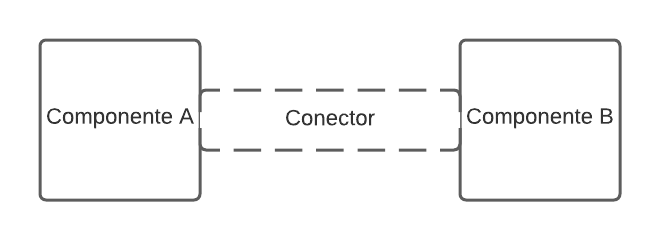
\includegraphics[scale=0.78]{03_arquitectura/images/conector}
  \caption{Ejemplo de comunicación de dos componentes a través de un conector.}
  \label{fig:componentesYConectorEjemplo}
\end{figure}

Internamente, los conectores están compuestos por uno o más \textbf{conductos} o canales. A través de estos se lleva a cabo la comunicación entre los componentes. Hay una gran variedad de conductos posibles: comunicación interproceso, a través de la red, etc. Clasificamos los conectores según la complejidad de los canales que utilizan \cite{mehtaTaxonomySoftwareConnectors2000}:

\begin{itemize}
    \item \textbf{Conectores simples}: solo cuentan con un conducto, sin lógica asociada. Son conectores sencillos. Suelen estar ya implementados en los lenguajes de programación. Por ejemplo: una llamada a función en un programa o el sistema de entrada / salida de ficheros.

    \item \textbf{Conectores complejos}: cuentan con uno o más conductos. Se definen por composición a partir de múltiples conectores simples. Además, pueden contar con funcionalidad para manejar el flujo de datos y/o control. Suelen utilizarse importando \emph{frameworks} o librerías. Por ejemplo: un balanceador de carga que redirige peticiones a los nodos.
\end{itemize}

Por tanto, cuando hayamos decidido qué dos componentes deben comunicarse, es momento de evaluar cuál es el mecanismo de comunicación más adecuado. Basándonos en nuestros requisitos, la arquitectura ya definida, y los mecanismos de despliegue que queremos usar, elegimos el conector apropiado. Podemos ayudarnos de taxonomías como la de \cite{mehtaTaxonomySoftwareConnectors2000} o encontrar otras fuentes de inspiración.

\subsubsection{Forma}

\textcolor{red}{TODO}

\subsubsection{Justificación}

Una vez definidos los componentes, los conectores y las relaciones entre ellos, tendremos una representación del sistema. Pero se trata de una imagen incompleta. No cuenta con ciertos detalles del contexto que nos ayudan a entenderlo mejor. Un ejemplo podría ser qué alternativas se consideraron y por qué se descartaron en favor de la elegida. Tampoco contamos con detalles minuciosos que puedan guiar mejor la implementación.

Es decir, requerimos de un concepto adicional para describirlos en nuestra arquitectura: se trata de la \textbf{justificación}. \cite{perryFoundationsStudySoftware1992} Nos aporta detalles más precisos sobre el sistema que no se pueden representar como elementos o forma.

\subsection{Estilos arquitectónicos}

\textcolor{red}{Podemos agrupar decisiones principales.}
